\documentclass[conference]{IEEEtran}

\usepackage{graphicx}
\usepackage{amsmath}
\usepackage{booktabs}
\usepackage{hyperref}

\title{Single-Channel RF Source Separation: Baseline Comparison and Robustness Sweeps}

\author{\IEEEauthorblockN{DL-AIR Team Draft}
\IEEEauthorblockA{Single-channel reporting run prepared for course feedback}}

\begin{document}
\maketitle

\begin{abstract}
This report summarizes a single-channel RF source separation study using synthetic QPSK mixtures. We compare learned models against a FastICA baseline and evaluate both waveform recovery and symbol recovery. The reporting run uses one received complex channel with the mixture model $s_{mix}=s_{soi} + \alpha s_{int} + noise$, where $\alpha$ controls interference strength and noise is parameterized by SNR in dB. Across the tested sweep range, symbol recovery remained perfect for all learned models and the FastICA baseline, but waveform recovery differed substantially. The best reference waveform results came from the LSTM and IQ-CNN models, while FastICA had the weakest waveform quality. These results suggest that the current single-channel synthetic setting is still relatively easy from the standpoint of symbol decisions, so waveform metrics provide the more sensitive comparison signal.
\end{abstract}

\section{Introduction}
The project goal is to separate a signal of interest (SOI) and an interference signal from a received RF mixture while preserving the transmitted symbols. In the final project report, we want to compare learned models against a classical baseline and quantify how robustness changes as interference and noise increase. This document is the first near-final reporting pass for the single-channel case.

The key reporting question is: \emph{how much waveform degradation can occur before symbol recovery begins to fail?} To answer that question, we report both waveform metrics and symbol-level accuracy, and we perform sweeps over interference strength $\alpha$ and SNR in dB.

\section{Related Work}
FastICA is a standard classical baseline for blind source separation and provides a useful non-neural comparison point \cite{hyvarinen1999fastica}. For waveform separation quality, SDR-style metrics are widely used in blind source separation studies \cite{vincent2006bss}. The learned models evaluated here include recurrent and convolutional architectures motivated by sequence modeling \cite{hochreiter1997lstm} and encoder-decoder style separation networks \cite{ronneberger2015unet}.

\section{Models Used and Modifications}
The single-channel reporting run compares six systems:
\begin{itemize}
    \item \textbf{FastICA}: classical non-trained baseline.
    \item \textbf{Tiny}: small convolutional separator.
    \item \textbf{Linear}: 1x1 convolutional baseline.
    \item \textbf{Hybrid}: linear front-end plus residual temporal refinement.
    \item \textbf{LSTM}: bidirectional sequence model.
    \item \textbf{IQ-CNN}: U-Net style separator operating through an I/Q wrapper.
\end{itemize}

The learned models were trained under the same single-channel reporting configuration and then evaluated on identical sweep datasets. FastICA was evaluated directly as a baseline with no training step.

\section{Data Generation and Parameters}
For this report, the received mixture follows
\begin{equation}
    s_{mix} = s_{soi} + \alpha s_{int} + noise .
\end{equation}

The data used in this reporting run is \textbf{single-channel}. Internally, the one received complex mixture is represented as two real-valued I/Q channels for model input. Both the SOI and interference are QPSK sequences modulated onto distinct carrier bins so they remain structurally separable in a controlled setting.

The QPSK symbol alphabet used in the evaluation is shown in Fig.~\ref{fig:qpsk_alphabet}. The label mapping is
\begin{equation}
    0 \rightarrow \frac{1 + 1j}{\sqrt{2}},\quad
    1 \rightarrow \frac{-1 + 1j}{\sqrt{2}},\quad
    2 \rightarrow \frac{-1 - 1j}{\sqrt{2}},\quad
    3 \rightarrow \frac{1 - 1j}{\sqrt{2}}.
\end{equation}

The report training configuration used 12{,}000 training examples, 1{,}500 validation examples, 20 training epochs, and a reference training point of $\alpha = 1.0$ with SNR $=15$ dB. The robustness sweeps then evaluated wider ranges of $\alpha$ and SNR on fixed held-out datasets.

\begin{figure}[t]
    \centering
    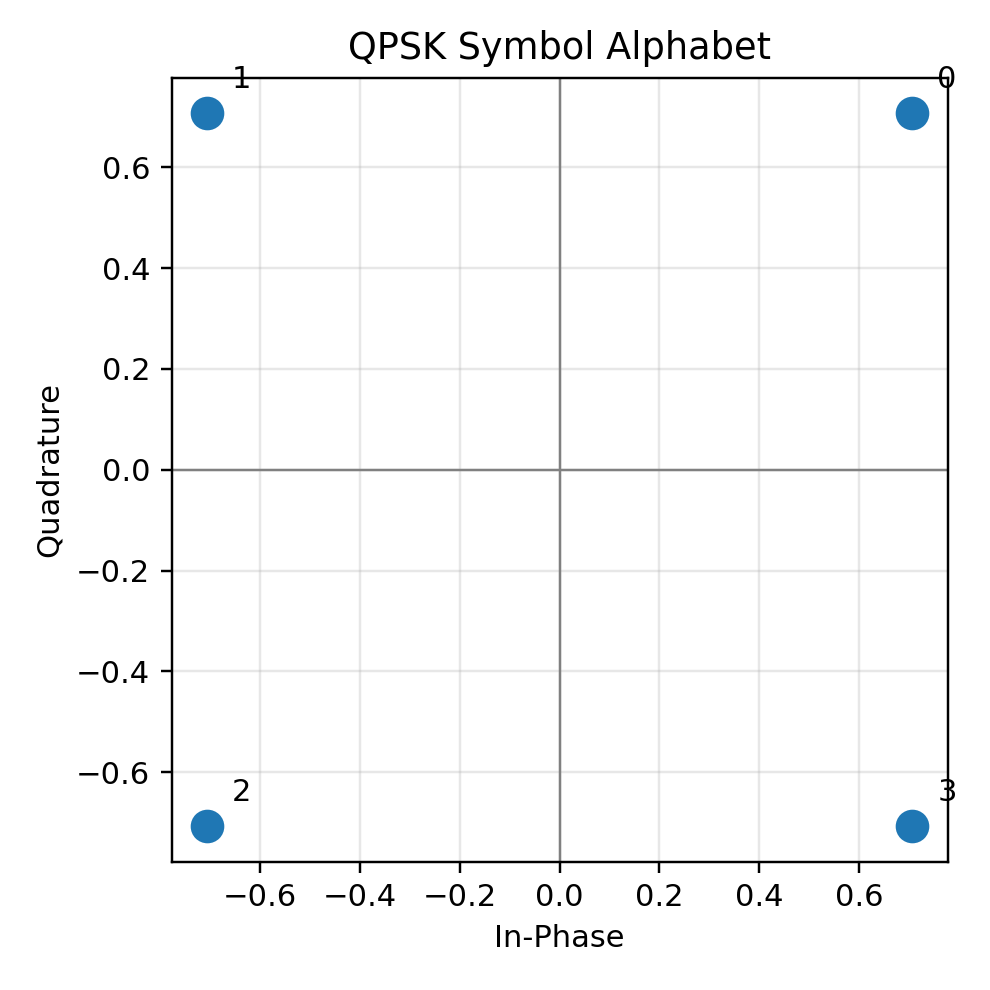
\includegraphics[width=0.9\columnwidth]{figures/qpsk_symbol_alphabet.png}
    \caption{QPSK symbol alphabet used in the single-channel reporting run.}
    \label{fig:qpsk_alphabet}
\end{figure}

\section{Evaluation Setup}
We report both waveform and symbol metrics.
\begin{itemize}
    \item \textbf{PIT-MSE}: permutation-invariant mean squared error between separated outputs and ground-truth sources.
    \item \textbf{Wave MSE}: direct waveform mean squared error after source alignment.
    \item \textbf{SDR}: signal-to-distortion ratio in dB.
    \item \textbf{SOI / interference symbol accuracy}: fraction of correctly recovered QPSK symbols for each source.
\end{itemize}

The final reporting pipeline generates:
\begin{itemize}
    \item one reference model-comparison table,
    \item an $\alpha$ robustness sweep,
    \item an SNR robustness sweep,
    \item wave-error versus symbol-accuracy visualizations,
    \item example signal figures for a learned model and the FastICA baseline.
\end{itemize}

\section{Reference Comparison Results}
Table~\ref{tab:model_comparison_reference} shows the reference comparison at $\alpha = 1.0$. In this setting, all methods achieved perfect symbol accuracy, so waveform metrics provide the more meaningful ranking.

\begin{table}[t]
\centering
\caption{Reference comparison on the fixed single-channel evaluation set.}
\label{tab:model_comparison_reference}
\begin{tabular}{|c|c|c|c|c|c|}
\hline
Model & PIT-MSE & Wave MSE & SDR & SOI Acc & Int Acc \\ 
\hline
FastICA & 0.6670 & 0.6670 & -1.16 & 1.000 & 1.000 \\ 
Tiny & 0.0755 & 0.0755 & 8.26 & 1.000 & 1.000 \\ 
Linear & 0.2589 & 0.2589 & 2.88 & 1.000 & 1.000 \\ 
Hybrid & 0.0319 & 0.0319 & 12.20 & 1.000 & 1.000 \\ 
LSTM & 0.0210 & 0.0210 & 14.17 & 1.000 & 1.000 \\ 
IQ\_CNN & 0.0240 & 0.0240 & 13.51 & 1.000 & 1.000 \\ 
\hline
\end{tabular}
\end{table}


Among the learned models, the LSTM achieved the lowest reference PIT-MSE (0.0210) and the highest SDR (14.17 dB). IQ-CNN followed closely with PIT-MSE 0.0240 and SDR 13.51 dB. Hybrid also performed strongly. FastICA was much weaker in waveform fidelity, with PIT-MSE 0.6670 and negative SDR, but still retained perfect symbol recovery in this simplified single-channel setting.

Figure~\ref{fig:ref_wave_mse} and Fig.~\ref{fig:ref_symbol_acc} show the same reference result from two perspectives: waveform quality and symbol accuracy.

\begin{figure}[t]
    \centering
    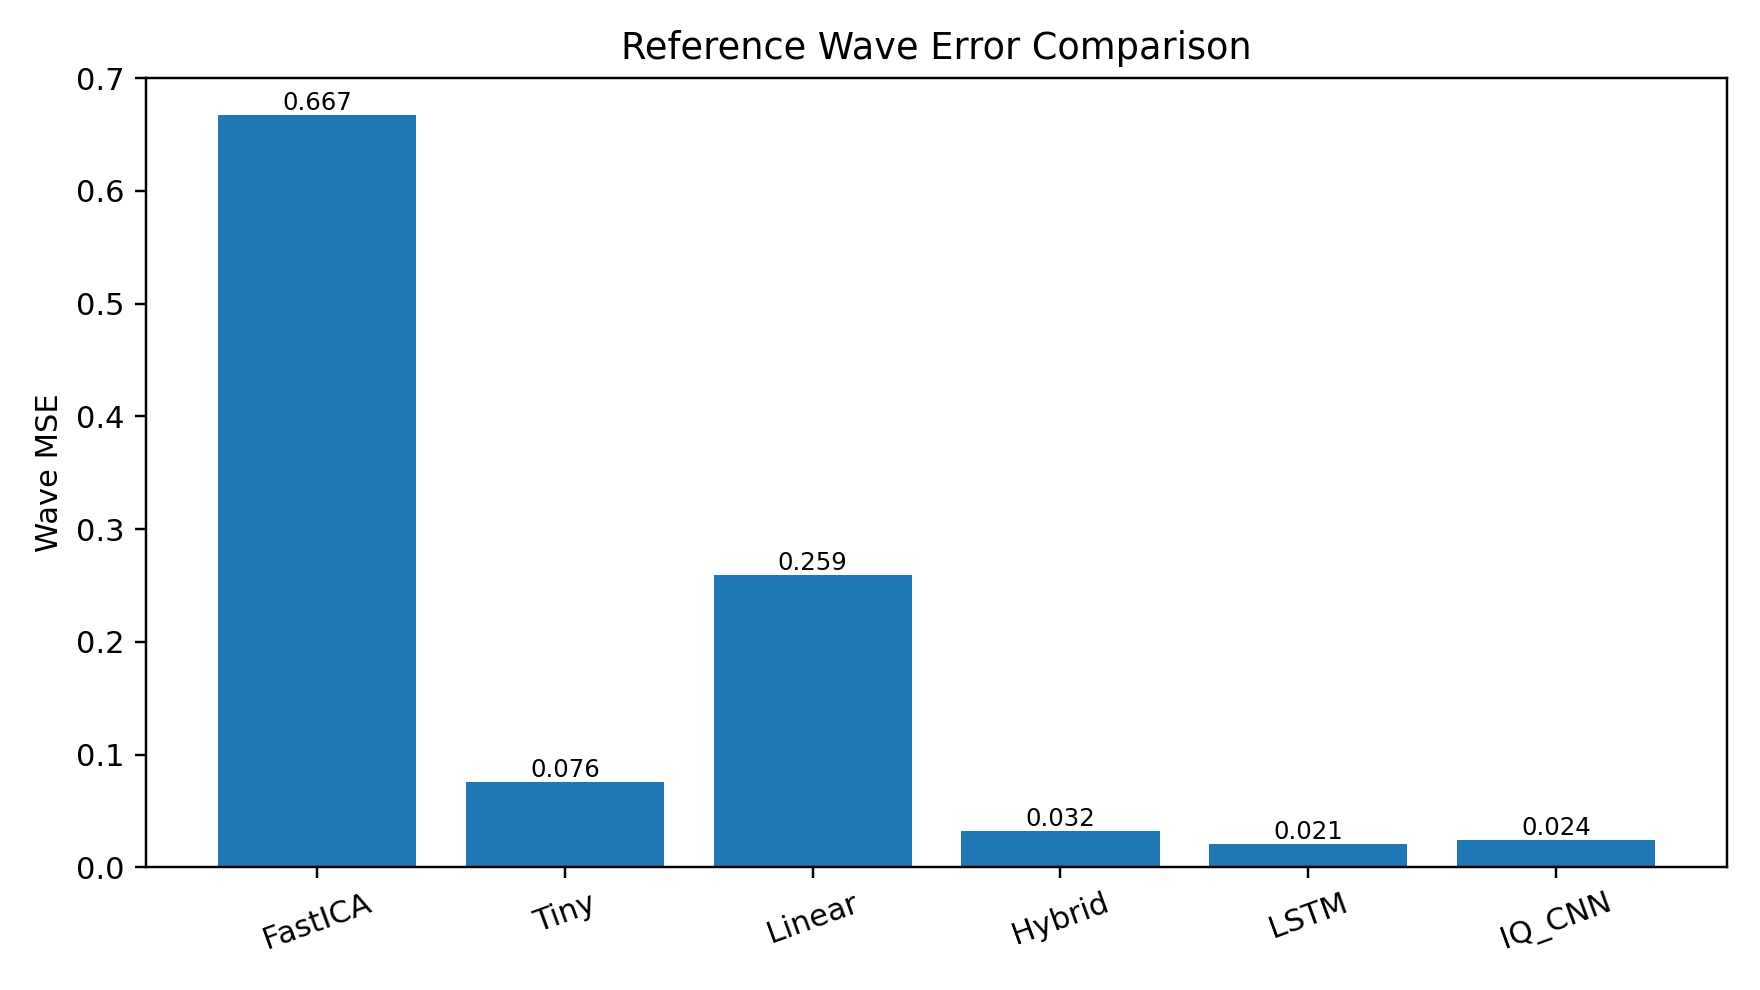
\includegraphics[width=0.95\columnwidth]{figures/model_comparison_reference_wave_mse.png}
    \caption{Reference comparison of wave MSE at $\alpha=1.0$. Lower is better.}
    \label{fig:ref_wave_mse}
\end{figure}

\begin{figure}[t]
    \centering
    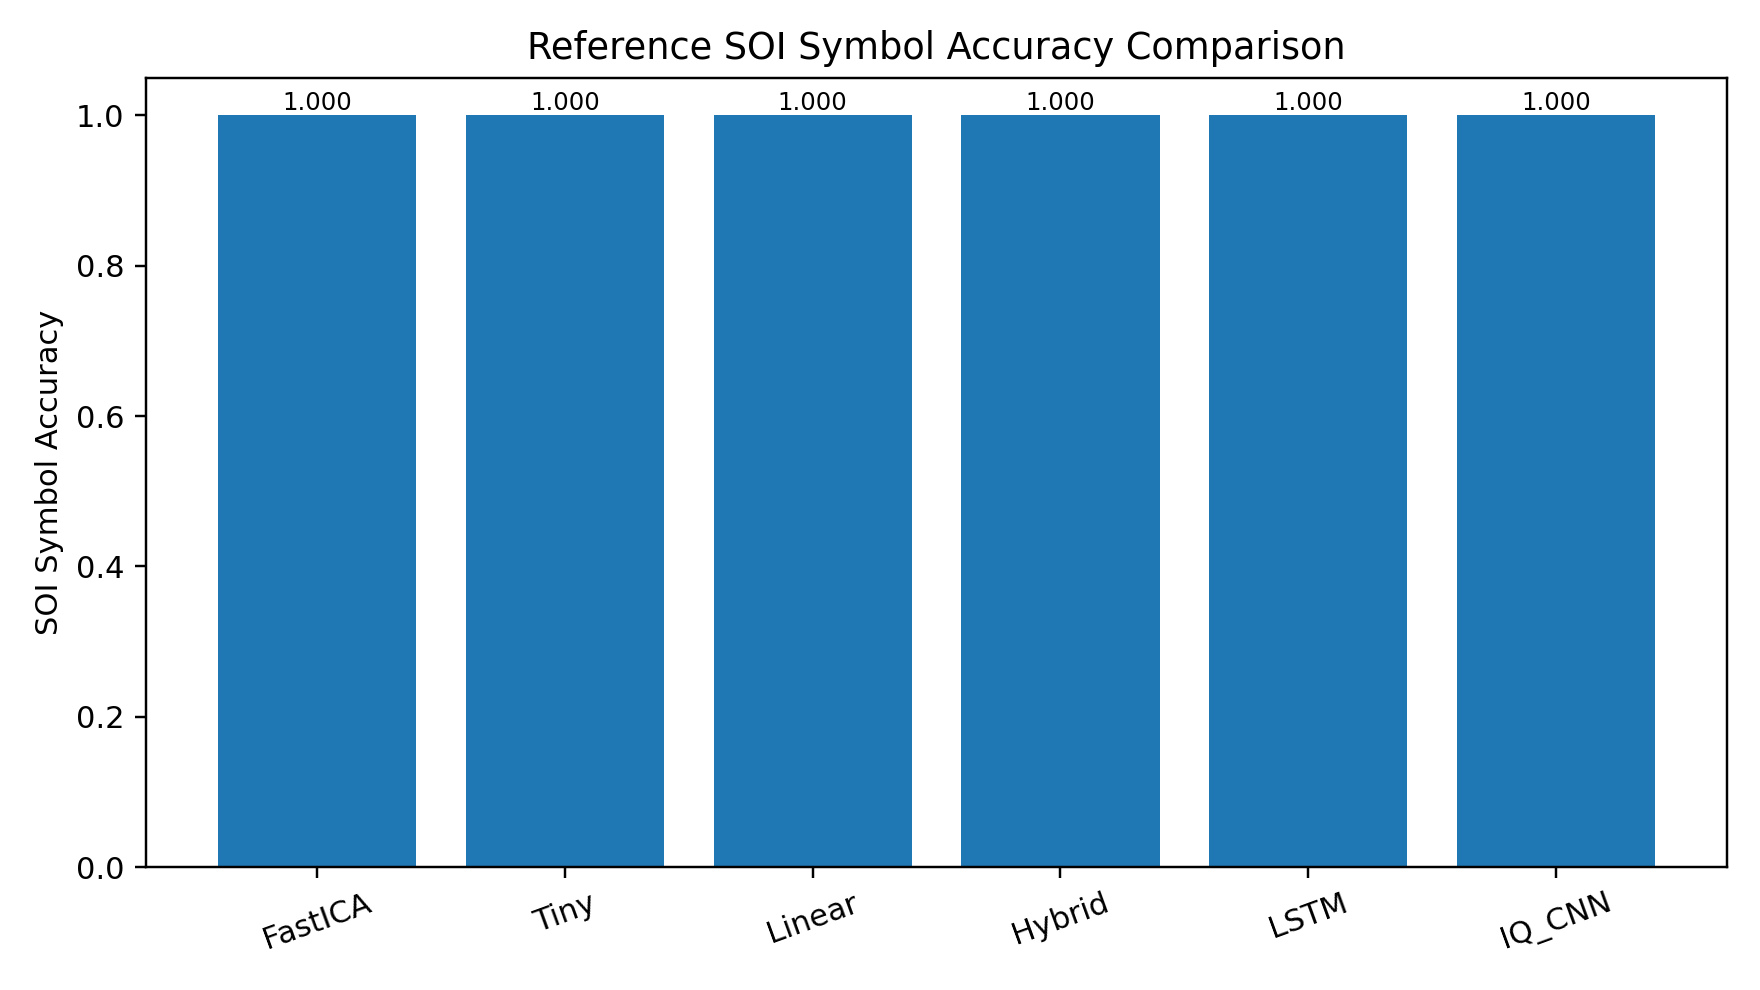
\includegraphics[width=0.95\columnwidth]{figures/model_comparison_reference_soi_accuracy.png}
    \caption{Reference comparison of SOI symbol accuracy at $\alpha=1.0$. In this setting, all tested methods reached perfect symbol recovery.}
    \label{fig:ref_symbol_acc}
\end{figure}

\section{Robustness to Interference Strength}
The first sweep increased interference strength through $\alpha$ while holding noise at the report reference level. Table~\ref{tab:alpha_robustness} summarizes the largest tested $\alpha$ before the SOI symbol accuracy dropped below 95\%.

\begin{table}[t]
\centering
\caption{Largest tested interference level before substantial SOI symbol degradation.}
\label{tab:alpha_robustness}
\begin{tabular}{|c|c|c|c|}
\hline
Model & Alpha & SOI Acc & Wave MSE \\ 
\hline
FastICA & 64.00 & 1.000 & 0.7172 \\ 
Hybrid & 64.00 & 1.000 & 201.8437 \\ 
IQ\_CNN & 64.00 & 1.000 & 0.5419 \\ 
LSTM & 64.00 & 1.000 & 0.4254 \\ 
Linear & 64.00 & 1.000 & 420.7559 \\ 
Tiny & 64.00 & 1.000 & 489.8495 \\ 
\hline
\end{tabular}
\end{table}


In the current single-channel setting, no learned model lost SOI symbol recovery anywhere in the tested $\alpha$ range, and even FastICA remained above the 95\% threshold. However, the waveform metrics separated the models clearly. Figure~\ref{fig:alpha_wave} shows that waveform error increased dramatically for the weaker models as interference grew, while LSTM and IQ-CNN degraded more slowly. Figure~\ref{fig:alpha_symbol} shows that symbol accuracy remained saturated despite large waveform differences.

\begin{figure}[t]
    \centering
    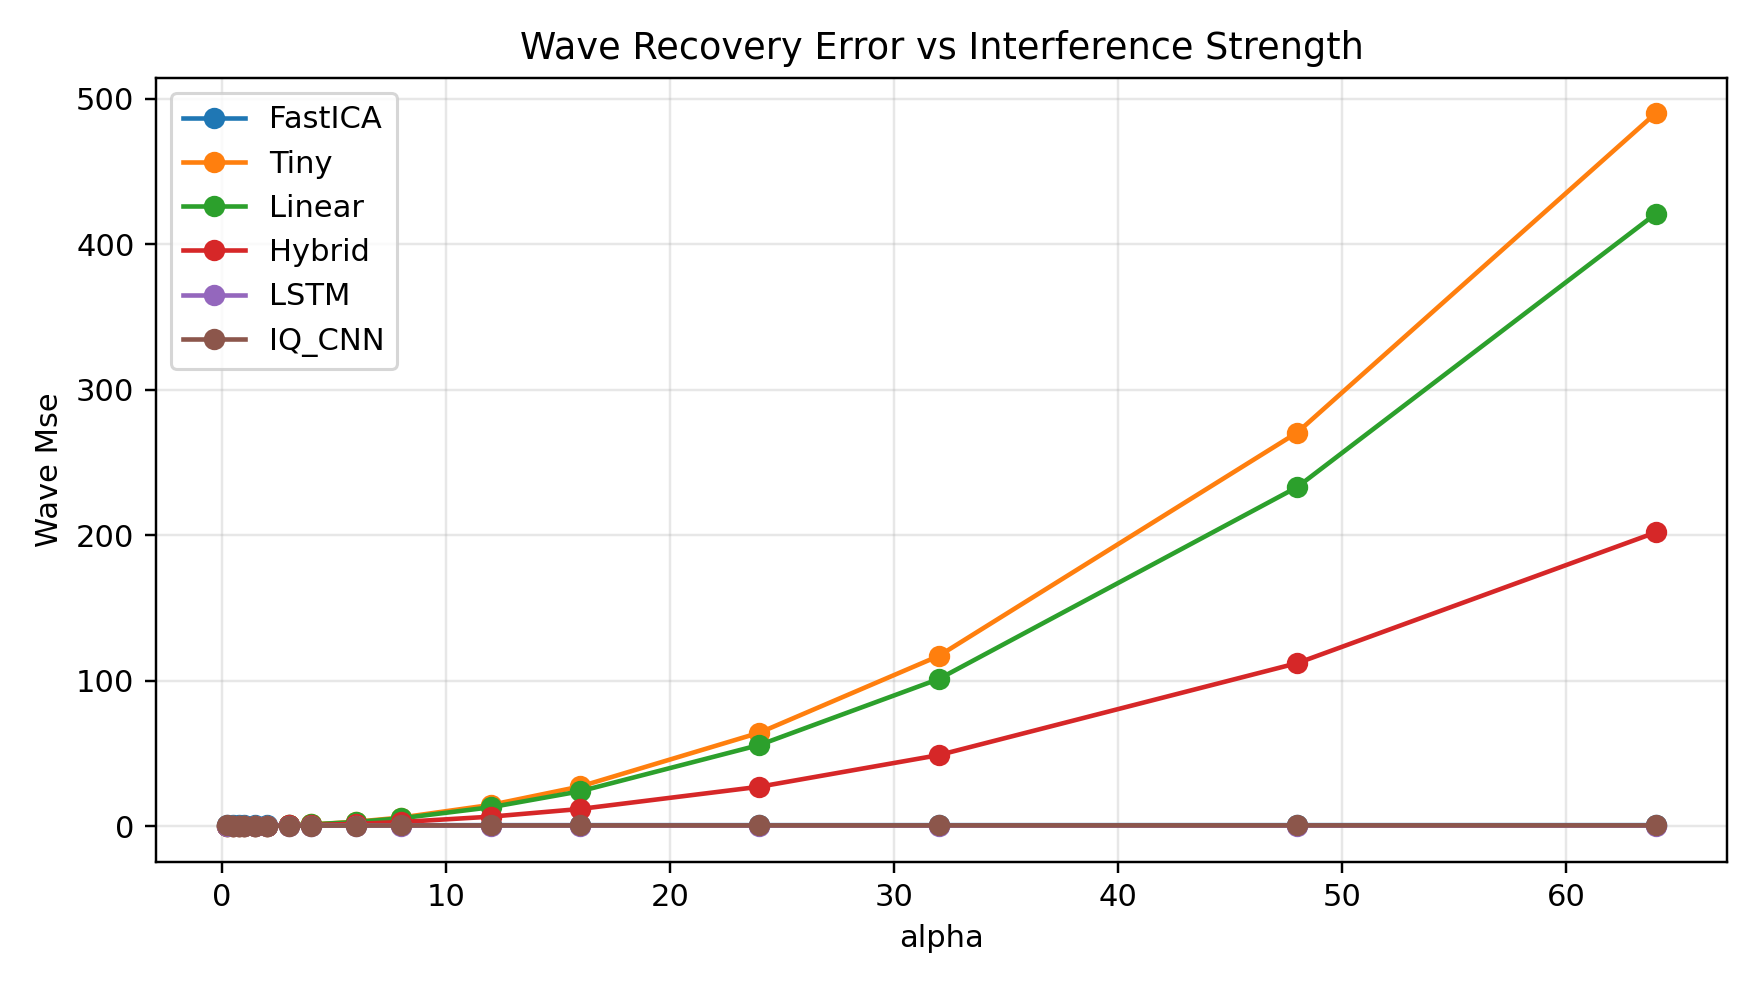
\includegraphics[width=0.95\columnwidth]{figures/alpha_sweep_wave_mse.png}
    \caption{Wave MSE as interference strength $\alpha$ increases. The learned models separate more cleanly than FastICA in waveform space.}
    \label{fig:alpha_wave}
\end{figure}

\begin{figure}[t]
    \centering
    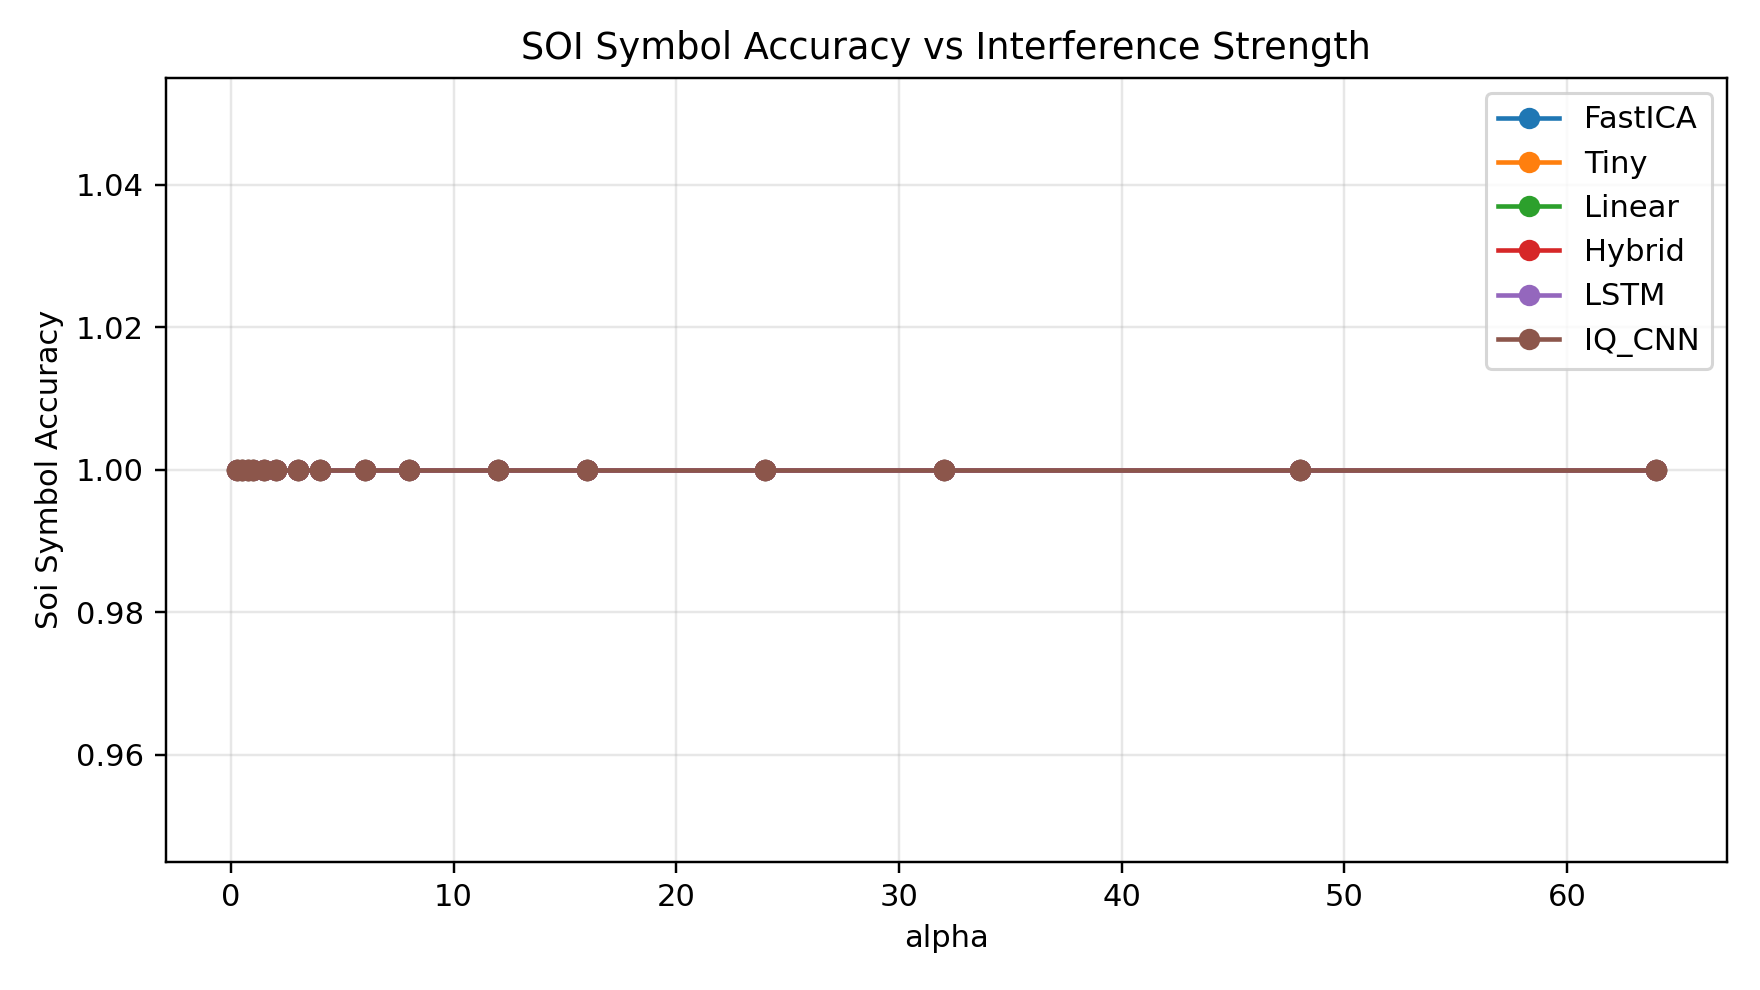
\includegraphics[width=0.95\columnwidth]{figures/alpha_sweep_soi_symbol_accuracy.png}
    \caption{SOI symbol accuracy as $\alpha$ increases. Symbol recovery stayed saturated across the tested range, even while waveform quality diverged.}
    \label{fig:alpha_symbol}
\end{figure}

\section{Robustness to Noise}
The second sweep reduced SNR while holding $\alpha = 1.0$. Table~\ref{tab:noise_robustness} summarizes the lowest tested SNR before SOI symbol accuracy dropped below 95\%.

\begin{table}[t]
\centering
\caption{Lowest tested SNR before substantial SOI symbol degradation.}
\label{tab:noise_robustness}
\begin{tabular}{|c|c|c|c|}
\hline
Model & SNR (dB) & SOI Acc & Wave MSE \\ 
\hline
FastICA & -30.0 & 1.000 & 0.9820 \\ 
Hybrid & -30.0 & 1.000 & 83.5601 \\ 
IQ\_CNN & -30.0 & 1.000 & 0.8498 \\ 
LSTM & -30.0 & 1.000 & 0.7605 \\ 
Linear & -30.0 & 1.000 & 235.0156 \\ 
Tiny & -30.0 & 1.000 & 323.8002 \\ 
\hline
\end{tabular}
\end{table}


Again, within the tested sweep range, all methods maintained near-perfect or perfect symbol recovery. The useful differentiation came from waveform quality. Figure~\ref{fig:noise_wave} shows that FastICA and the simpler models degrade much more quickly in waveform space as noise increases, whereas the best learned models remain substantially better. Figure~\ref{fig:noise_symbol} shows that symbol decisions remain robust down to the lowest tested SNR values in this controlled single-channel case.

\begin{figure}[t]
    \centering
    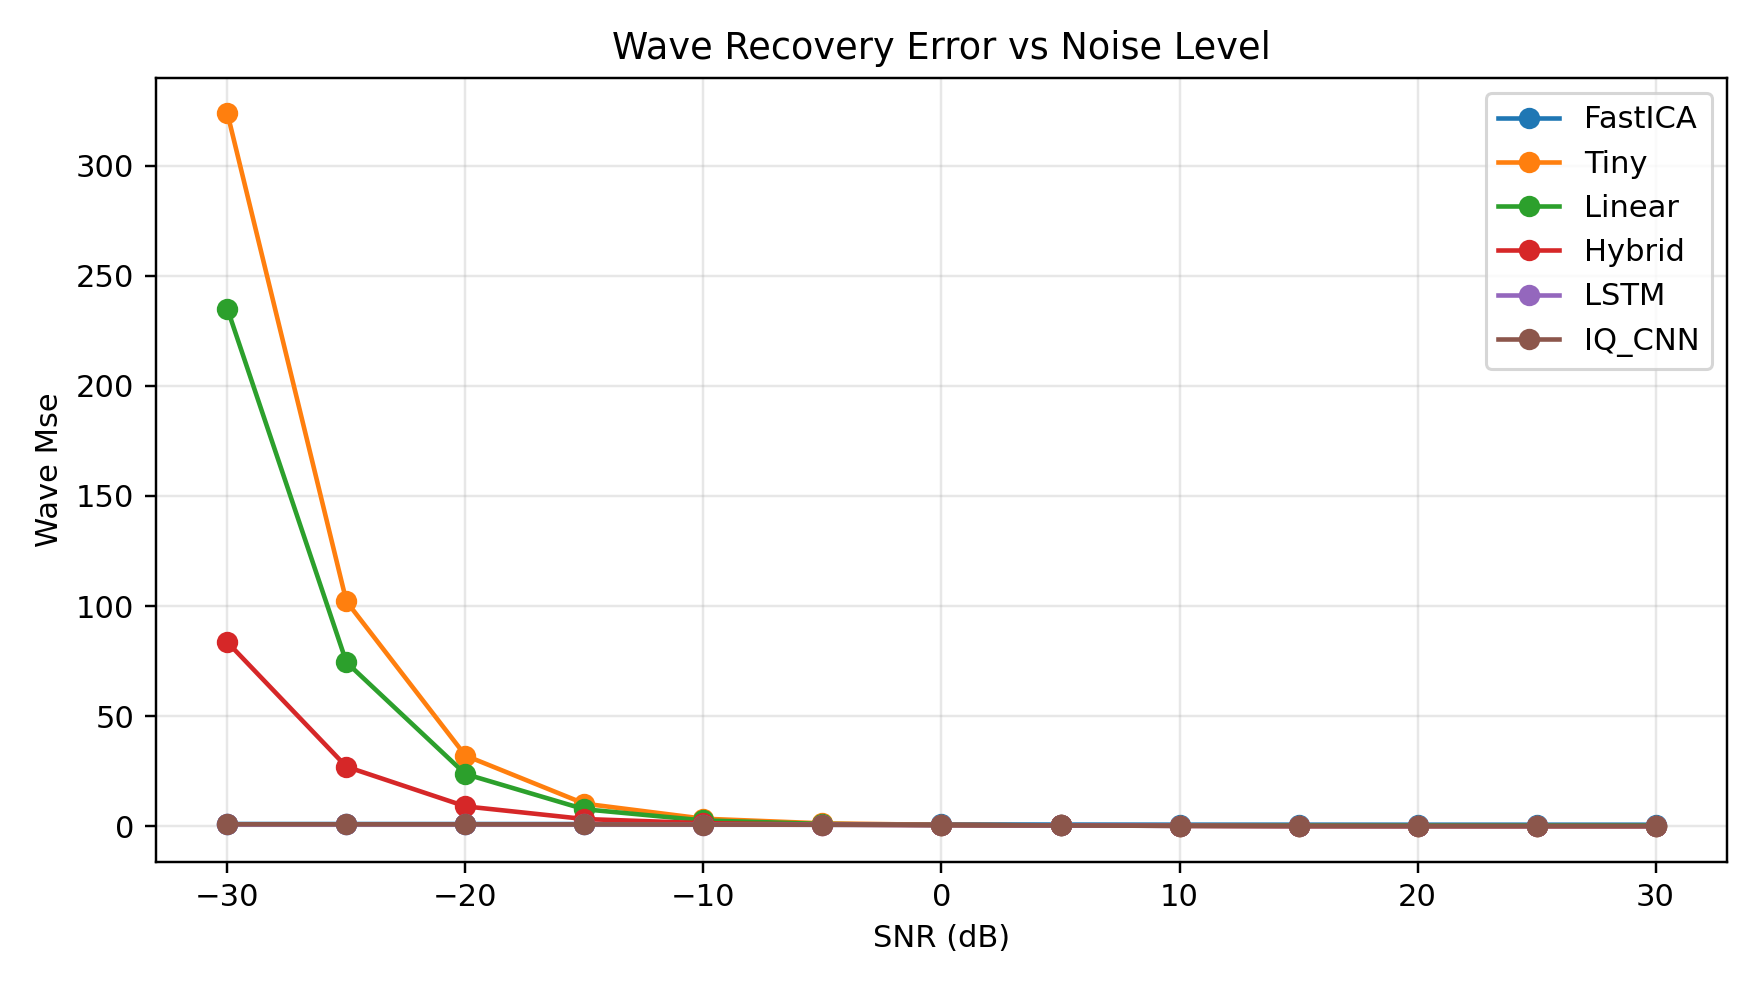
\includegraphics[width=0.95\columnwidth]{figures/noise_sweep_wave_mse.png}
    \caption{Wave MSE as SNR decreases. Waveform degradation is visible well before symbol accuracy collapses.}
    \label{fig:noise_wave}
\end{figure}

\begin{figure}[t]
    \centering
    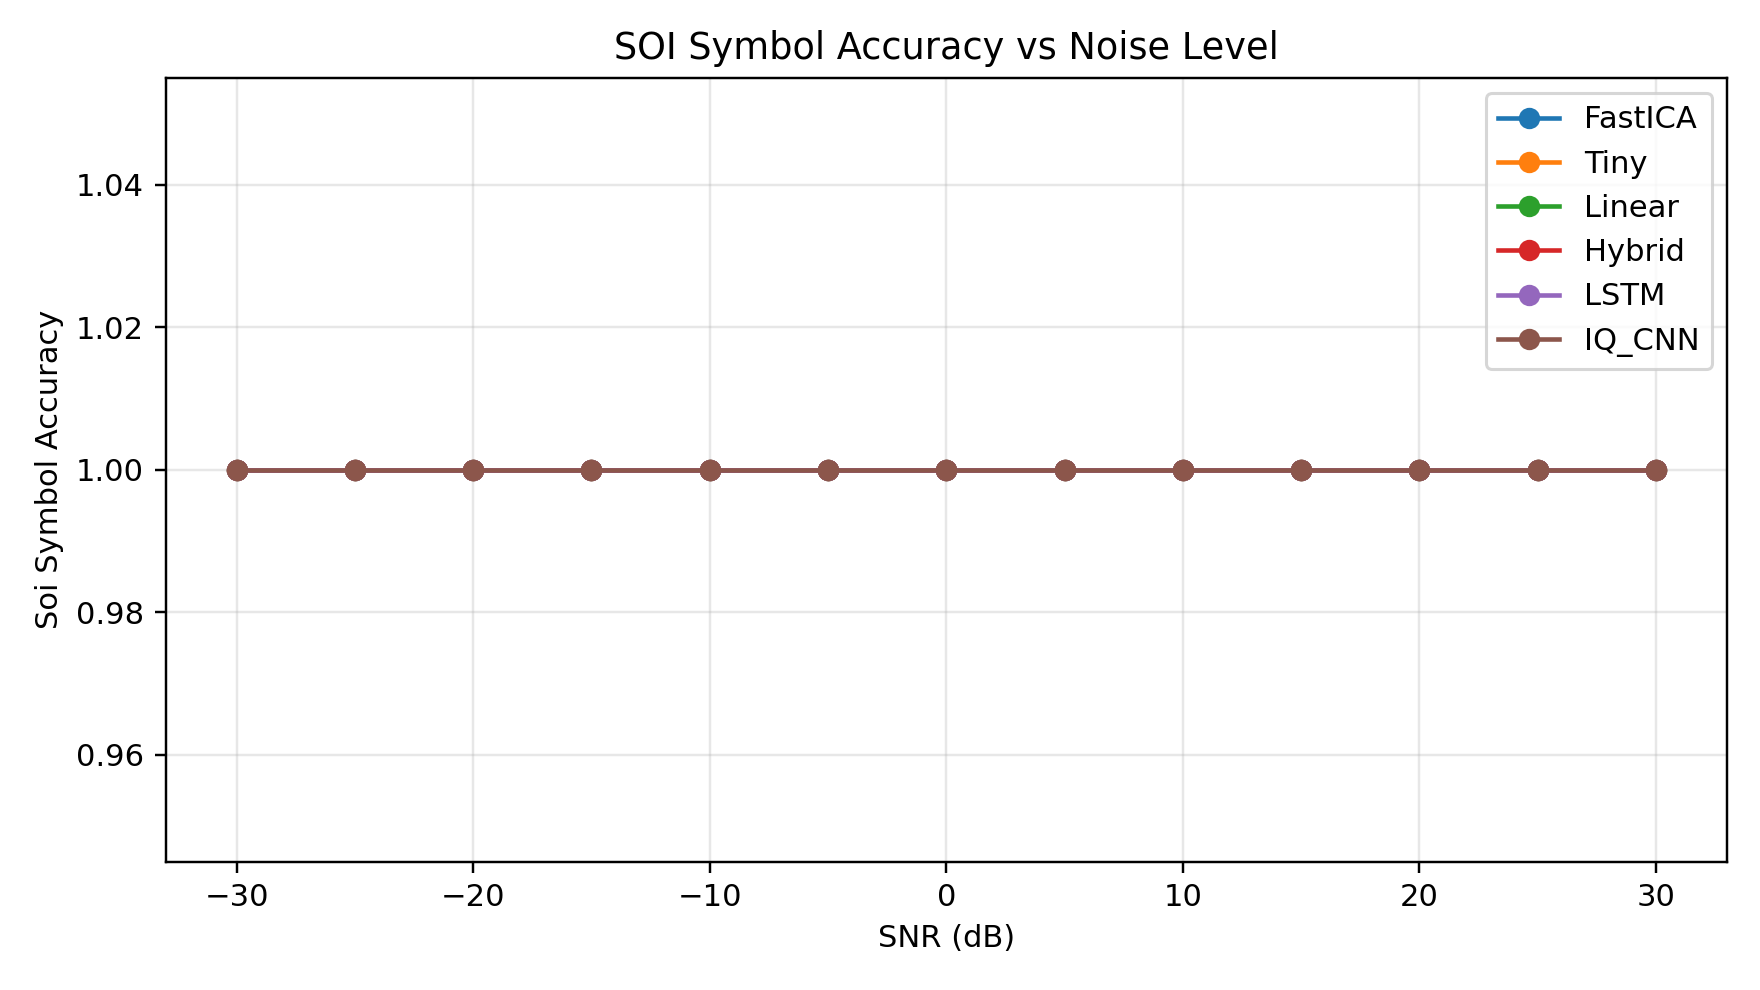
\includegraphics[width=0.95\columnwidth]{figures/noise_sweep_soi_symbol_accuracy.png}
    \caption{SOI symbol accuracy as SNR decreases. The current single-channel synthetic setting remains symbol-robust over the tested range.}
    \label{fig:noise_symbol}
\end{figure}

\section{Wave Recovery Versus Symbol Recovery}
One of the central goals of this project is to understand how much waveform error can be tolerated before symbol recovery begins to fail. Figures~\ref{fig:wave_symbol_alpha} and~\ref{fig:wave_symbol_noise} show that, in the present single-channel evaluation, symbol accuracy remains saturated even as wave MSE changes substantially across models and sweep conditions.

This is an important finding: for this easier single-channel setting, waveform metrics are currently more informative than symbol metrics for ranking model quality. In other words, the tested conditions are still not difficult enough to expose symbol-level failure for the learned models.

\begin{figure}[t]
    \centering
    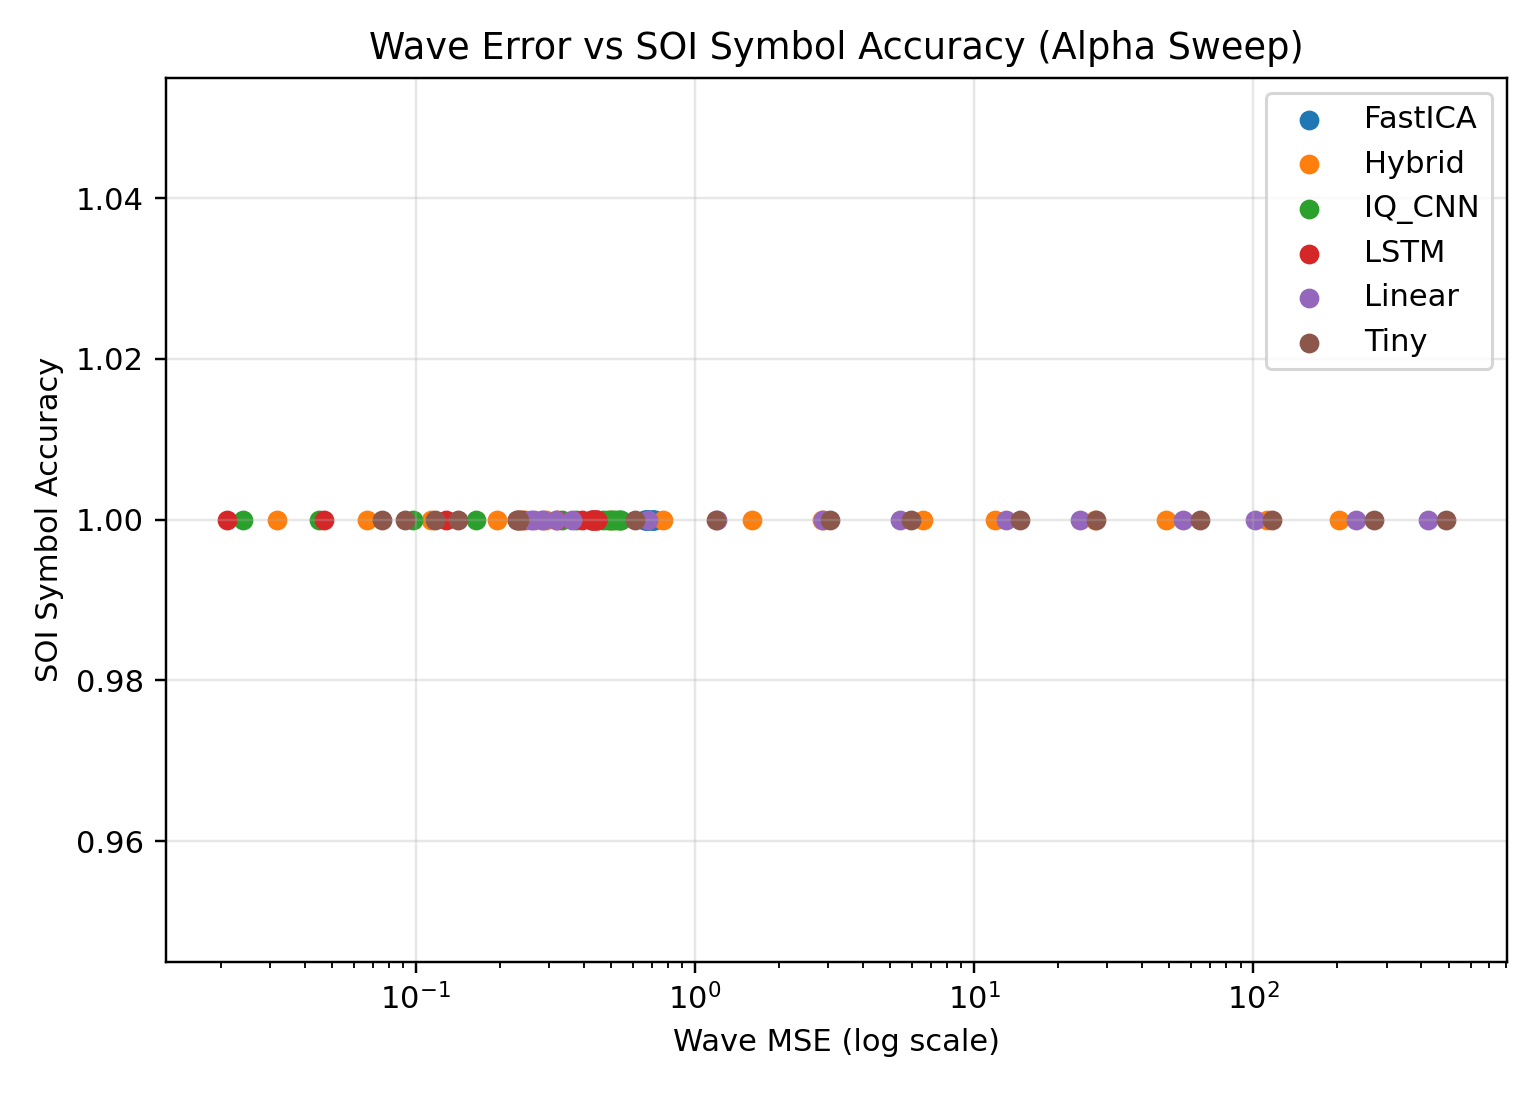
\includegraphics[width=0.95\columnwidth]{figures/wave_error_vs_symbol_accuracy_alpha.png}
    \caption{Relationship between wave error and SOI symbol accuracy during the interference sweep.}
    \label{fig:wave_symbol_alpha}
\end{figure}

\begin{figure}[t]
    \centering
    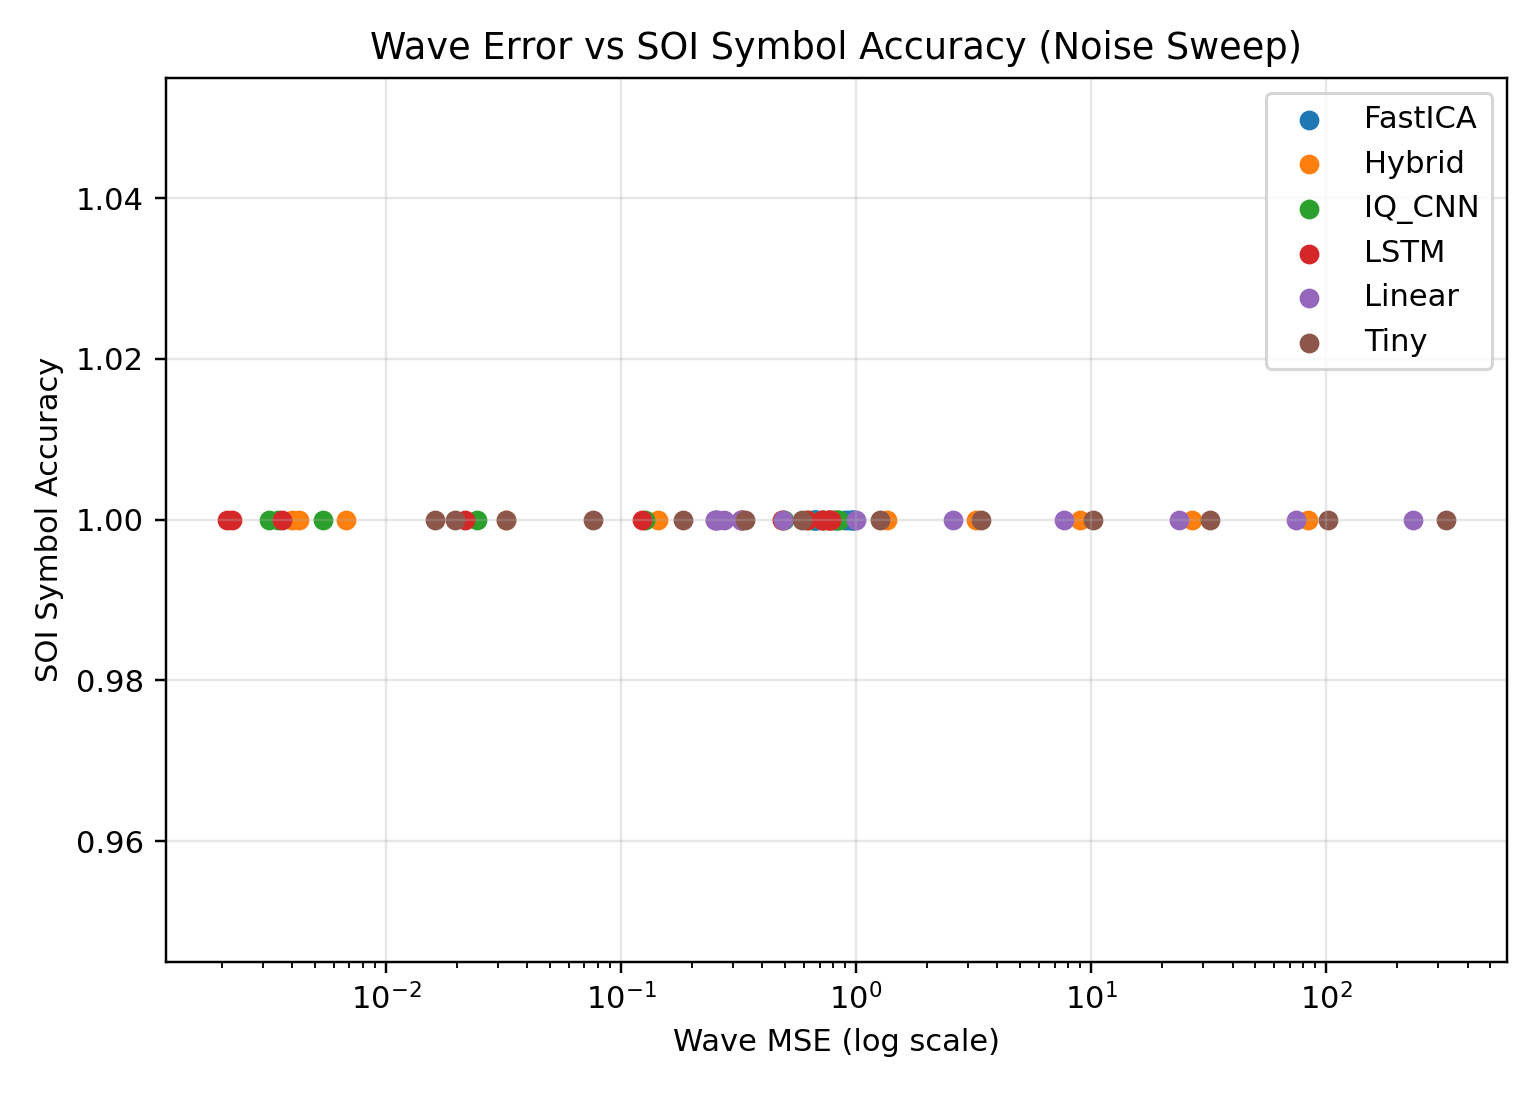
\includegraphics[width=0.95\columnwidth]{figures/wave_error_vs_symbol_accuracy_noise.png}
    \caption{Relationship between wave error and SOI symbol accuracy during the noise sweep.}
    \label{fig:wave_symbol_noise}
\end{figure}

\section{Example Signals}
Figures~\ref{fig:best_example} and~\ref{fig:fastica_example} provide concrete examples of what the system is separating. Each figure shows clean sources, the received mixture, and the separated outputs. The learned-model example demonstrates visibly cleaner waveform recovery than the FastICA baseline, even though both can still decode the symbol stream in this controlled setting.

\begin{figure}[t]
    \centering
    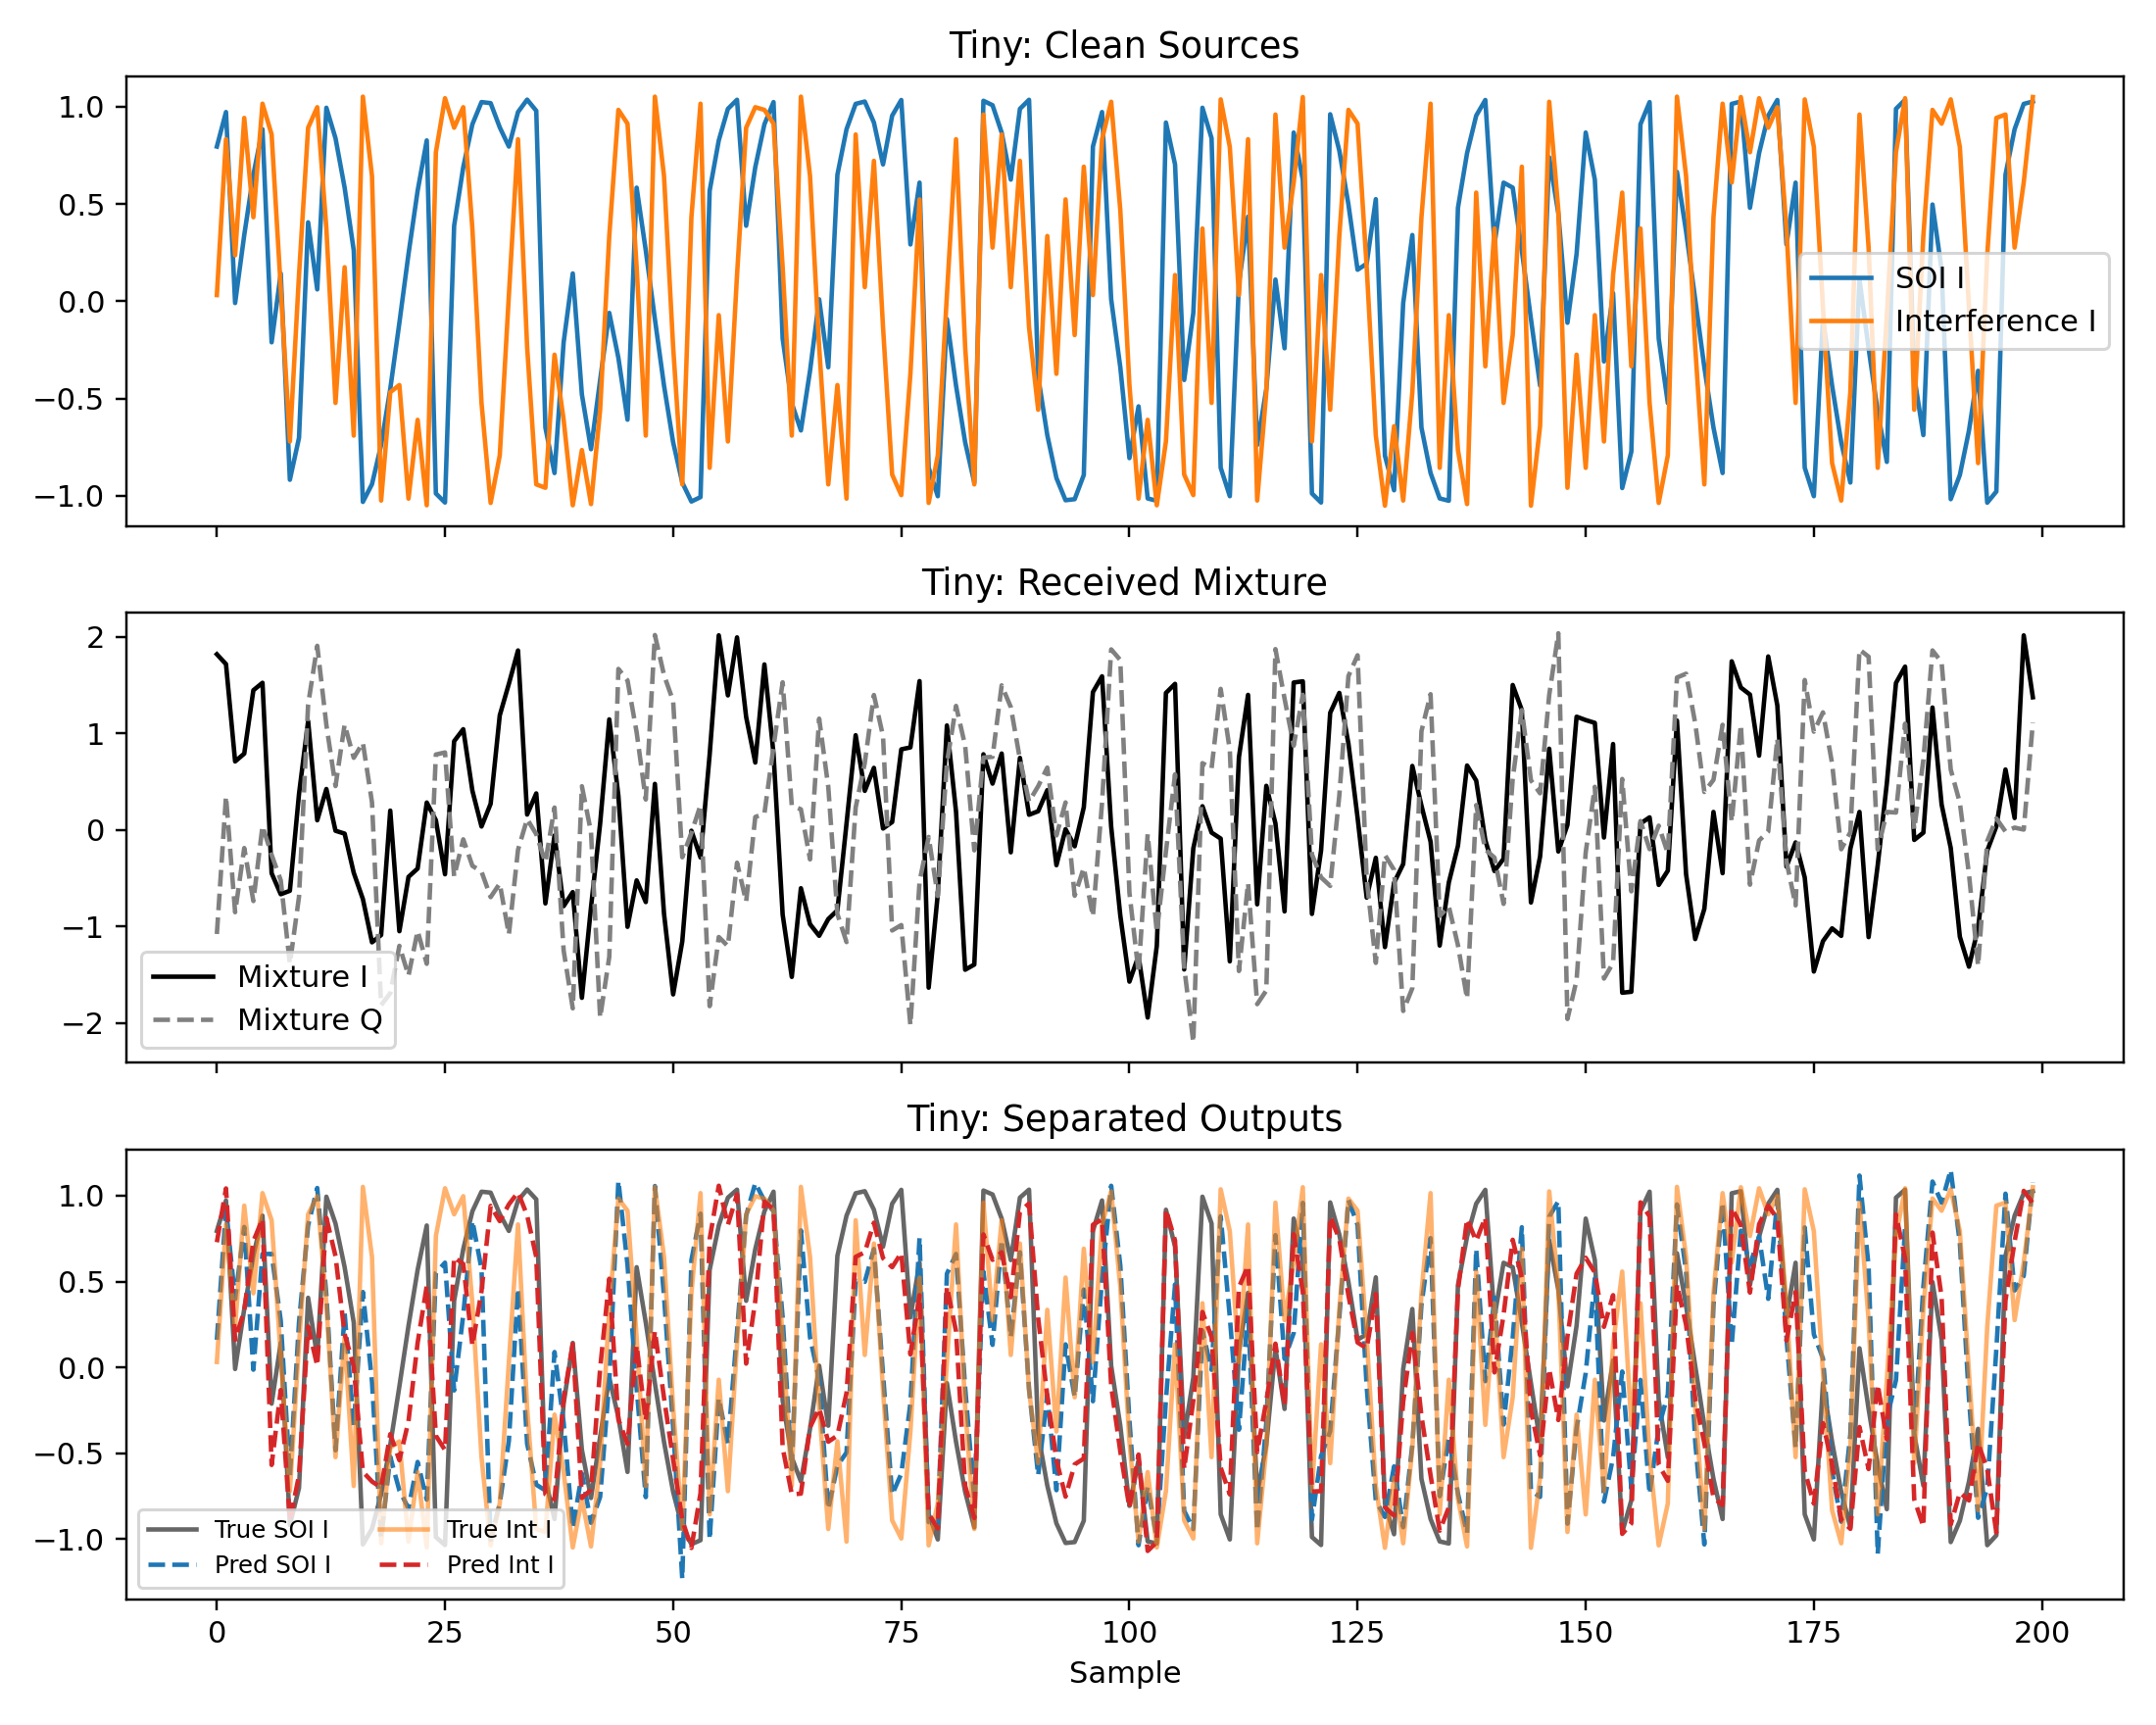
\includegraphics[width=0.95\columnwidth]{figures/pipeline_example_best_model.png}
    \caption{Example source, mixture, and output visualization for the best learned model in the reference comparison.}
    \label{fig:best_example}
\end{figure}

\begin{figure}[t]
    \centering
    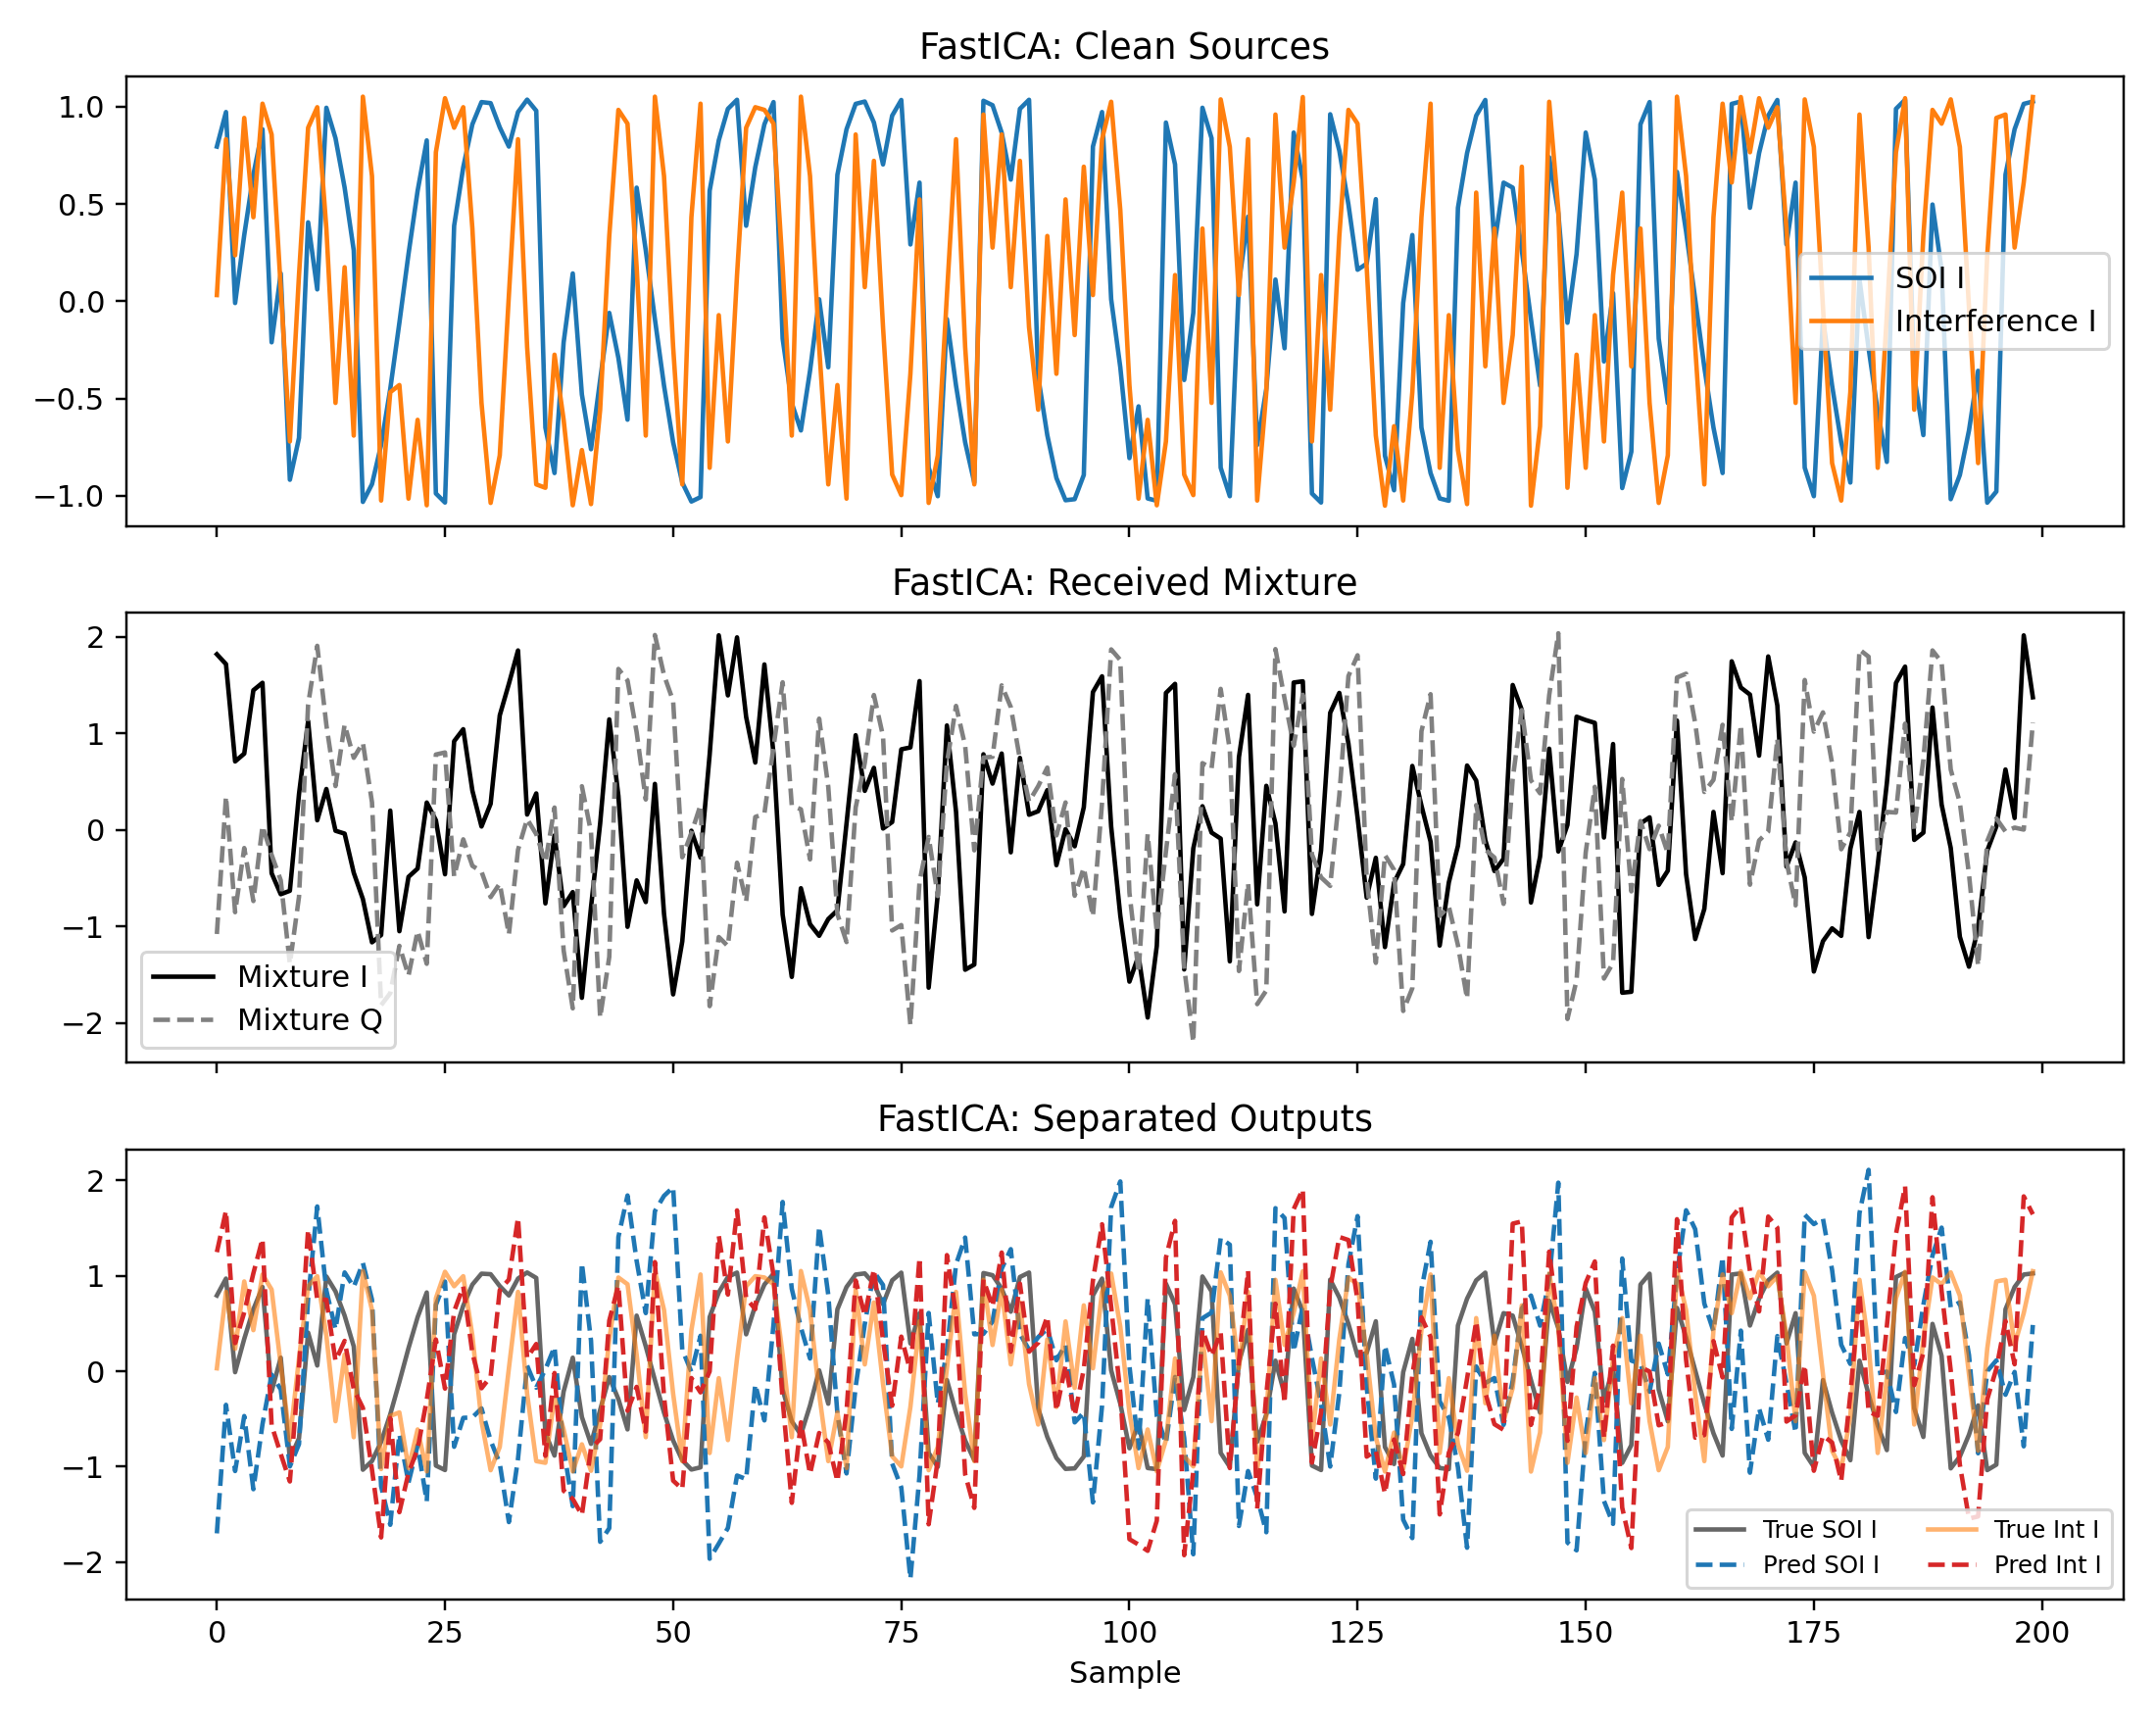
\includegraphics[width=0.95\columnwidth]{figures/pipeline_example_fastica.png}
    \caption{Example source, mixture, and output visualization for the FastICA baseline.}
    \label{fig:fastica_example}
\end{figure}

\section{Conclusion}
This single-channel reporting run produced three main conclusions. First, the learned models outperform FastICA in waveform recovery, with the LSTM and IQ-CNN producing the strongest reference results. Second, the current single-channel synthetic setting is still easy enough that all learned models preserve perfect symbol recovery across the tested interference and noise sweeps, and even FastICA remains symbol-robust. Third, waveform error is therefore the more sensitive metric for comparing models in this setting.

The main implication is that the next reporting step should move to a harder setting, such as a more challenging single-channel generator or the planned four-channel receiver case. That will help identify the point where symbol recovery finally begins to degrade and make the robustness study more discriminative.

\bibliographystyle{IEEEtran}
\bibliography{references/references}

\appendices
\section{Appendix}
The appendix can be expanded later with the full sweep tables, implementation details, and additional examples. The current report folder already includes the generated tables and figures needed for that extension.

\end{document}
